\documentclass[10pt]{article}
\usepackage{fontspec}
\usepackage{polyglossia}
\setdefaultlanguage{french}
\usepackage[a4paper,margin=2cm]{geometry}
\usepackage{url,hyperref}
\usepackage{siunitx}
\usepackage{schemabloc}
\usepackage{listings}
\usepackage{auto-pst-pdf}
\usepackage{pst-circ}
\usepackage{soul}
\usepackage{verbatim}
\usepackage{lmodern}
\usepackage{tikz}
\usepackage[european,cuteinductors,siunitx]{circuitikz}
\usepackage{xunicode,xltxtra}
\usepackage{graphicx}
\usepackage{amsmath}
\usepackage{minted}
\usepackage{multicol}
\usepackage{float}
\floatplacement{figure}{H}
\title{
\includegraphics{../../../images/inp-enseeiht} \\ ~ \\ ~ \\ ~ \\ ~ \\
TP Hyperfréquences \\ ~ \\ ADS}
\author{Matthieu Couffinhal, Guilhem Saurel}
\date{\today}
\renewcommand{\thesection}{\Roman{section}}
\renewcommand{\thesubsection}{\thesection .\alph{subsection}}
\begin{document}

\begin{titlepage}
    \maketitle
    \tableofcontents
\end{titlepage}

\part{Simulation non linéaire d’une chaîne de réception Bluetooth}
\section{Mise en œuvre d’une simulation Harmonic Balance}

\begin{figure}
    \begin{center}
        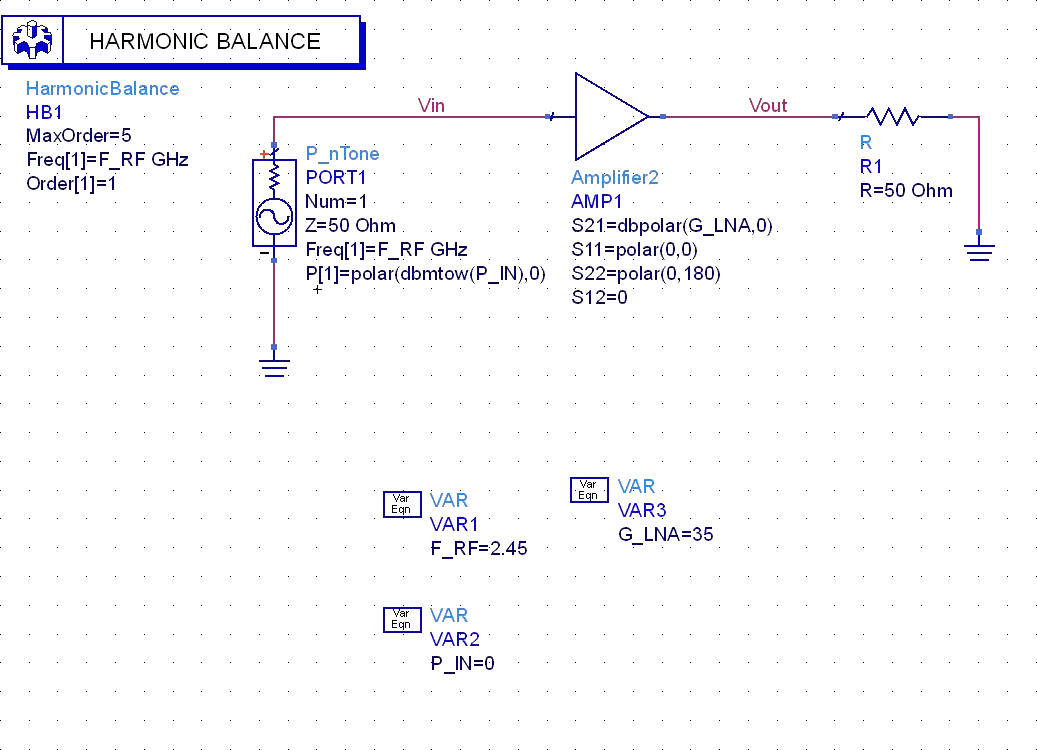
\includegraphics[width=15cm]{p5_circuit}
    \end{center}
    \caption{Circuit de test d’une Harmonic Balance}
\end{figure}

\begin{figure}
    \begin{center}
        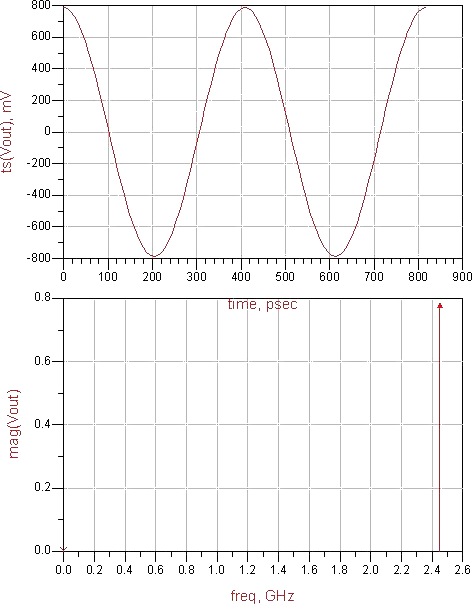
\includegraphics{p6_simu_1}
    \end{center}
    \caption{Réponse à l’ordre 1}
\end{figure}

On observe une raie à $f=2.45$Ghz d’amplitude 0.8V sur le spectre et une sinusoïde de période $T=1/f\simeq408$ms et d’amplitude 800mV sur la réponse temporelle.

En effet, le bruit est à 25dB en dessous du signal, donc on ne le voit pas.

L’amplitude de la tension observée vaut $V=\sqrt{PR}=\sqrt{P_{in}G_{LNA}R} = \sqrt{1\cdot 10^{-3}\cdot 10^{\cfrac{35}{20}}\cdot 50} \simeq 0.8$V

\begin{figure}
    \begin{center}
        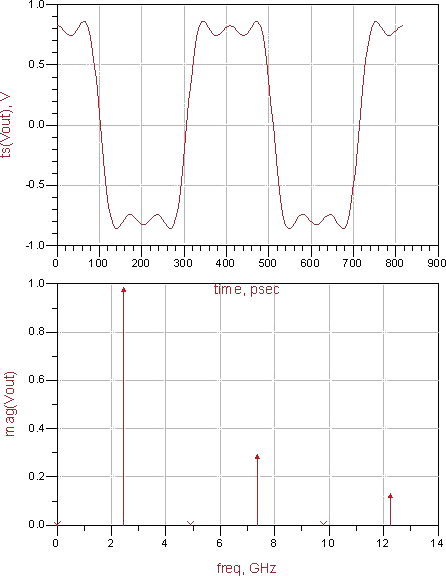
\includegraphics{p6_simu_5}
    \end{center}
    \caption{Réponse à l’ordre 5}
\end{figure}

Sur le domaine spectral, on observe clairement que deux raies se sont ajoutées à notre signal initial, à
$2.45\times 3=7.38$GHz et $2.45\times 5=12.25$GHz. Puisqu’on a ajouté des harmoniques de rang impair d’amplitudes décroissantes en $\cfrac{1}{n^2}$, la recomposition de ce signal est le développement limité à l’ordre 5 d’un carré. Et c’est bien ce que nous observons en temporel.

\section{Étude du mélangeur}

\begin{figure}
    \begin{center}
        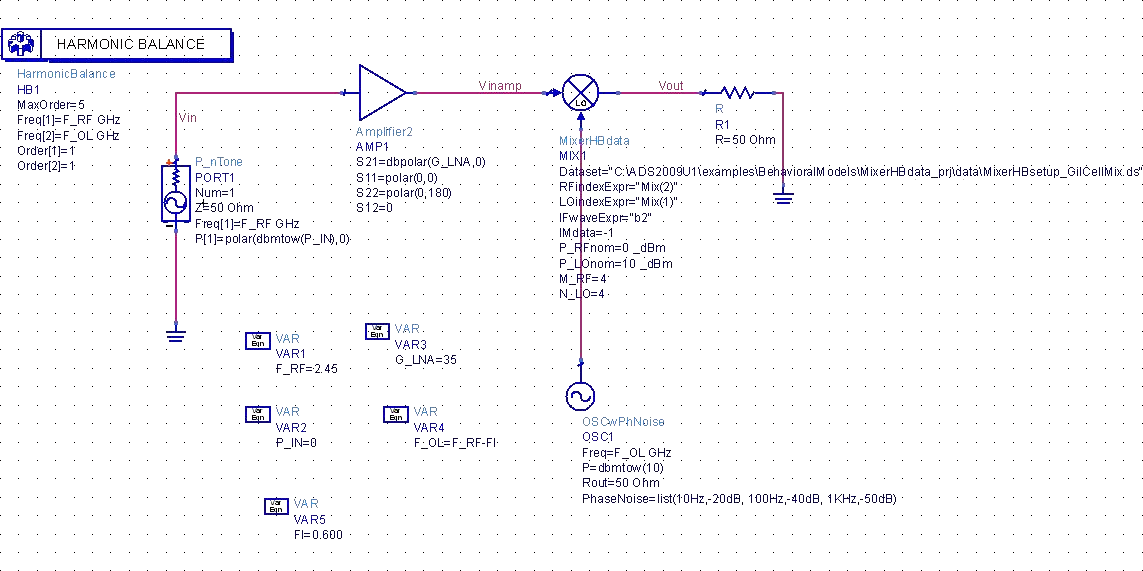
\includegraphics[width=15cm]{p8_circuit}
    \end{center}
    \caption{Mélangeur: calcul de $F_{OL}$ et circuit}
\end{figure}

\begin{figure}
    \begin{center}
        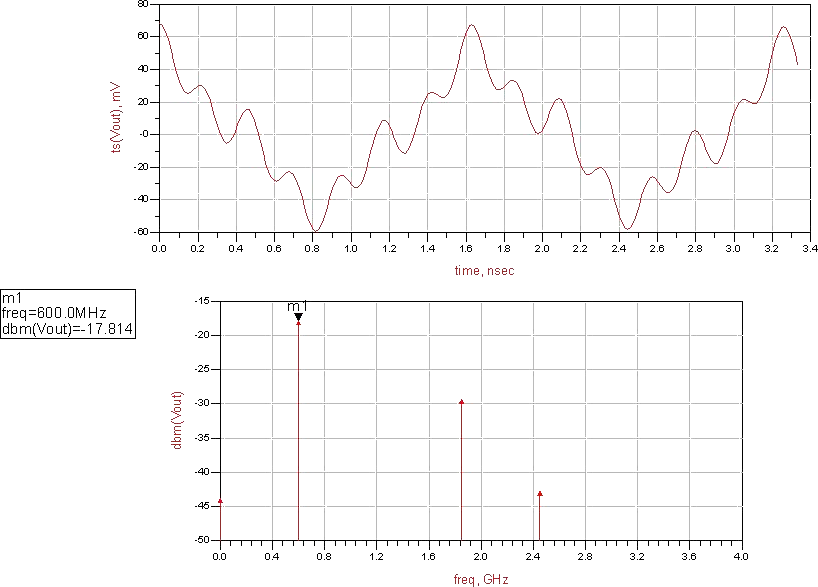
\includegraphics[width=15cm]{p8_simu_1}
    \end{center}
    \caption{Réponse du mélangeur à l’ordre 1}
\end{figure}

En sortie du mélangeur et au premier ordre, nous avons les fréquences 

$F_I=600$MHz, $F_{OL}=F_{RF}-F_I=1.85$GHz et $F_{RF}=2.45$GHz.

\begin{figure}
    \begin{center}
        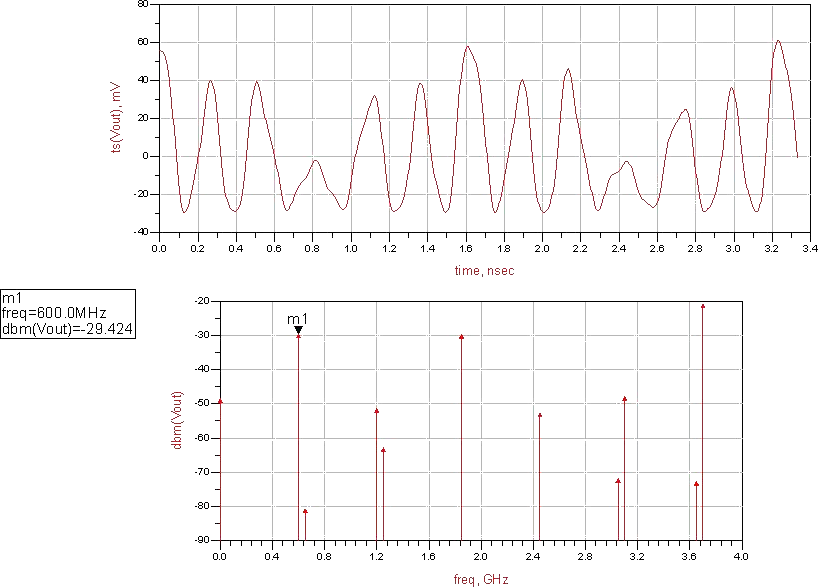
\includegraphics[width=15cm]{p8_simu_3}
    \end{center}
    \caption{Réponse du mélangeur à l’ordre 3}
\end{figure}

Les fréquences qui apparaissent entre 0 et 4GHz à l’ordre 3 sont:
\begin{itemize}
    \item $|0\times F_{RF}-2\times F_{OL}|=3.70$GHz;
    \item $|0\times F_{RF}-1\times F_{OL}|=1.85$GHz=$F_{OL}$;
    \item $|0\times F_{RF}+1\times F_{OL}|=1.85$GHz=$F_{OL}$;
    \item $|0\times F_{RF}+2\times F_{OL}|=3.70$GHz;
    \item $|1\times F_{RF}-3\times F_{OL}|=3.10$GHz;
    \item $|1\times F_{RF}-2\times F_{OL}|=1.25$GHz;
    \item $|1\times F_{RF}-1\times F_{OL}|=0.60$GHz=$F_I$;
    \item $|1\times F_{RF}+0\times F_{OL}|=2.45$GHz=$F_{RF}$;
    \item $|2\times F_{RF}-3\times F_{OL}|=0.65$GHz;
    \item $|2\times F_{RF}-2\times F_{OL}|=1.20$GHz;
    \item $|2\times F_{RF}-1\times F_{OL}|=3.05$GHz;
    \item $|3\times F_{RF}-3\times F_{OL}|=1.80$GHz;
    \item $|3\times F_{RF}-2\times F_{OL}|=3.65$GHz;
\end{itemize}

On peut encore augmenter l’ordre jusqu’à 5 avant d’obtenir une stabilité au niveau de puissance du signal:

\begin{figure}
    \begin{center}
        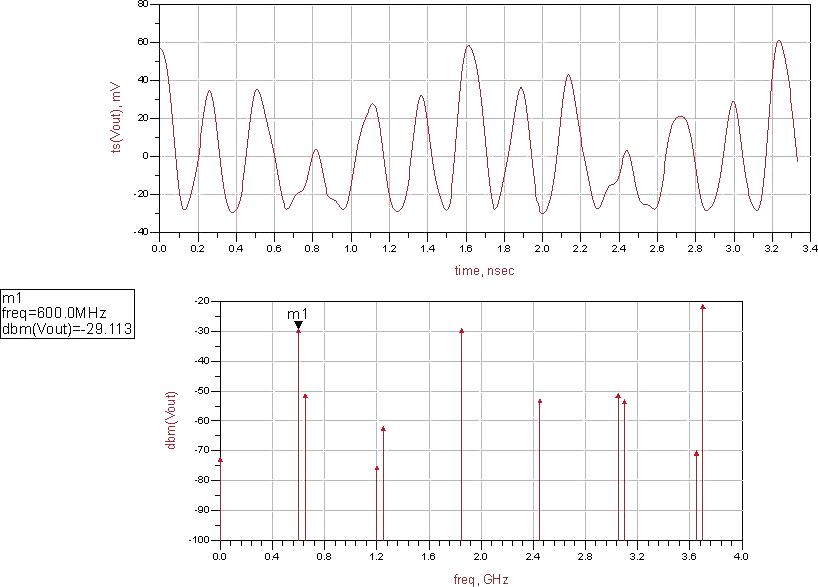
\includegraphics[width=15cm]{p8_simu_5}
    \end{center}
    \caption{Réponse du mélangeur à l’ordre 5}
\end{figure}

\section{Utilisation de fonctions de filtrage}

\begin{figure}
    \begin{center}
        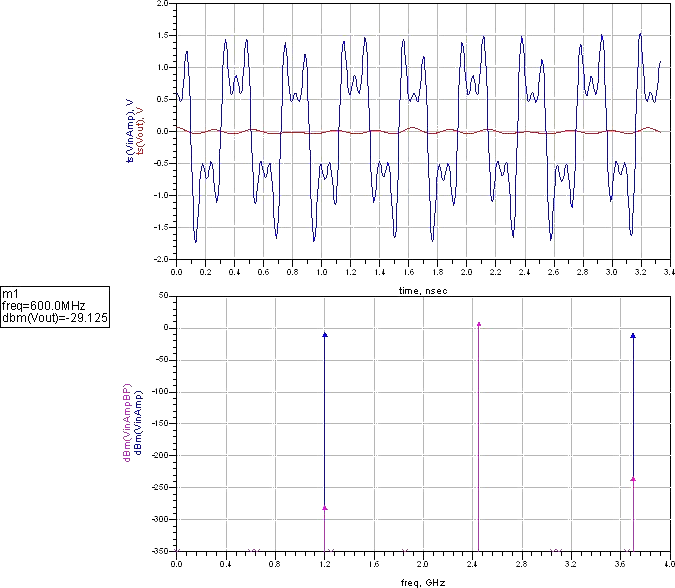
\includegraphics{p8_simu_circuit_2}
    \end{center}
    \caption{Simulation du mélangeur après ajout d’un filtre de Tchebycheff}
\end{figure}

Le diagramme spectral donne le signal initial amplifié \verb|VinAmp| et le même signal après passage dans
le filtre de Tchebycheff \verb|VinAmpBP|. Le résultat est clair: le premier a trois composantes à des 
amplitudes très proches, et le second est égal au premier, si ce n’est que les amplitudes des fréquences
qui ne nous intéressent pas ont été réduites de 200 à 300dBm.

\begin{figure}
    \begin{center}
        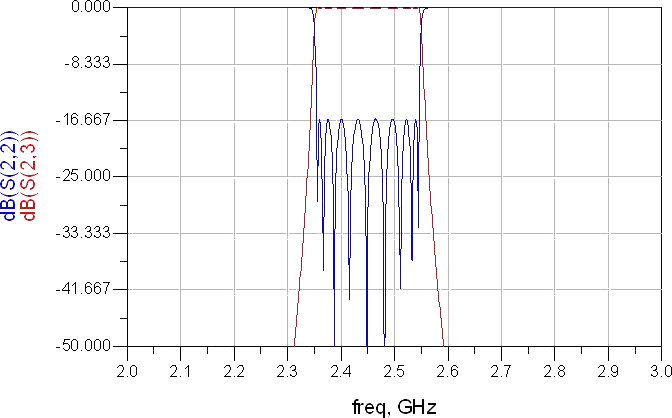
\includegraphics{p8_simu_ordre9_parametre_S}
    \end{center}
    \caption{Réponse du filtre (Paramètres S)}
\end{figure}

Vu l’allure du coefficient de réflexion, c’est un filtre du neuvième ordre.

\section{Simulation multi-ton}

\begin{figure}
    \begin{center}
        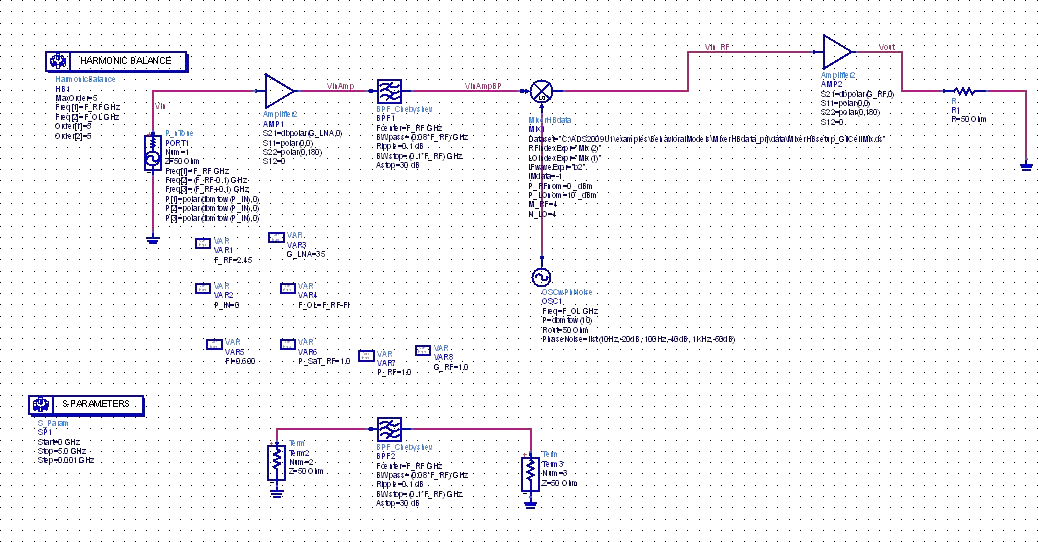
\includegraphics[width=15cm]{p10_circuit}
    \end{center}
    \caption{Circuit après prise en compte du multi-ton}
\end{figure}

\begin{figure}
    \begin{center}
        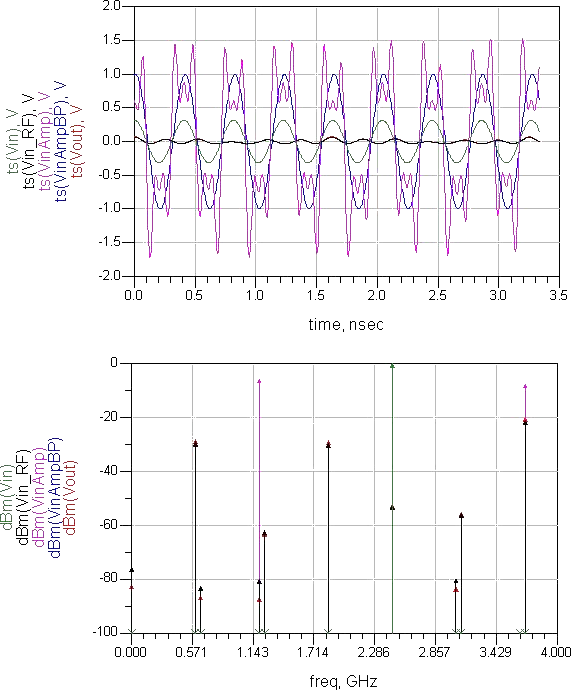
\includegraphics{p10_simu}
    \end{center}
    \caption{Simulation globale de la chaîne de réception BlueTooth}
\end{figure}

La sortie de notre filtre présente plusieurs fréquences parasites, donc notre filtre, qui était efficace
avec une seule fréquence d’entrée, est devenu inefficace lorsqu’on a pris en compte un signal d’entrée
avec des fréquences proches de celle qui nous intéresse et dont les amplitudes sont du même ordre.

\part{Conception de filtre passe-bande}
\section{Mise en œuvre}
\subsection{Prototype passe-bas}

Pour un filtre du troisième ordre avec 0.01dB de riple, les coefficients de Tchebycheff sont: 
$g_1=0.6291$, $g_2=0.9702$ et $g_3=1.0000$; la fréquence est de 2.45GHz, la pulsation de 
$\omega_0 = 2\pi\times 2.45\cdot10^9$rad/s, la bande passante de $2.45\times 0.18$Ghz et les valeurs dénormalisées
en fréquence et en impédance des composants de $C_1=\cfrac{g_1}{Z_0\omega_0}$, 
$L_2 = \cfrac{g_2Z_0}{\omega_0}$ et $C_3=\cfrac{g_3}{Z_0\omega_0}$.

\begin{figure}
    \begin{center}
        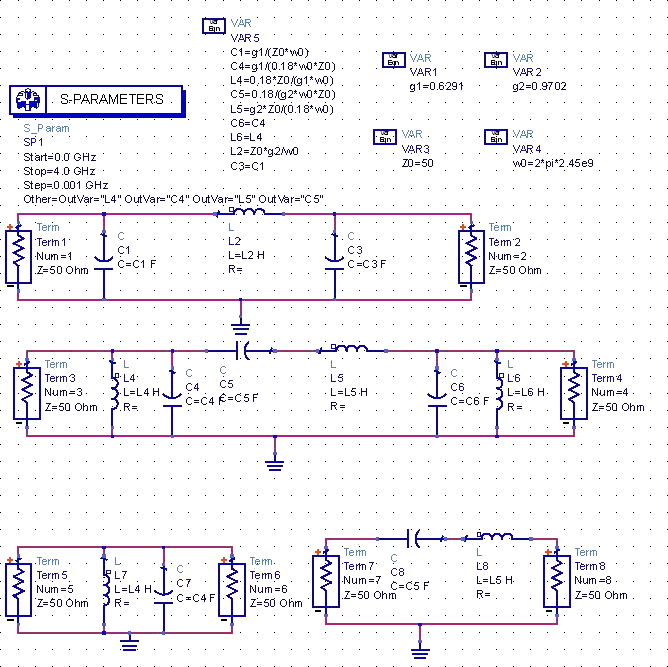
\includegraphics{p17_circuit}
    \end{center}
    \caption{Calculs et circuits passe-bas, passe bande, et résonnateurs seuls}
\end{figure}

\begin{figure}
    \begin{center}
        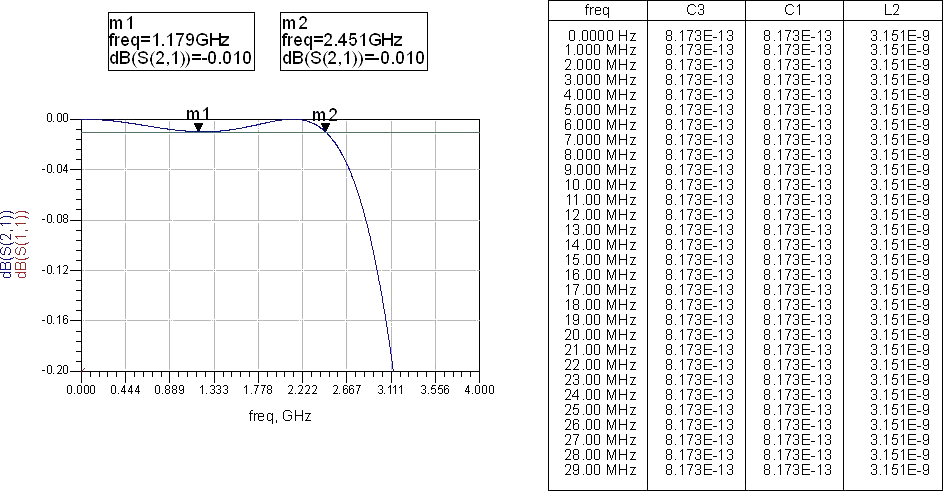
\includegraphics[width=15cm]{p17_simu}
    \end{center}
    \caption{Réponse du filtre passe-bas}
\end{figure}

On vérifie bien que les contraintes du cahier des charges sont respectées. Cependant, les valeurs des
composants (L \& C) ne sont pas tout à fait de l’ordre de grandeur des composants discrets que nous 
avons l’habitude de manipuler: ils ont des valeurs à peu près 1000 fois plus petites.

\subsection{Prototype passe-bande}

\begin{figure}
    \begin{center}
        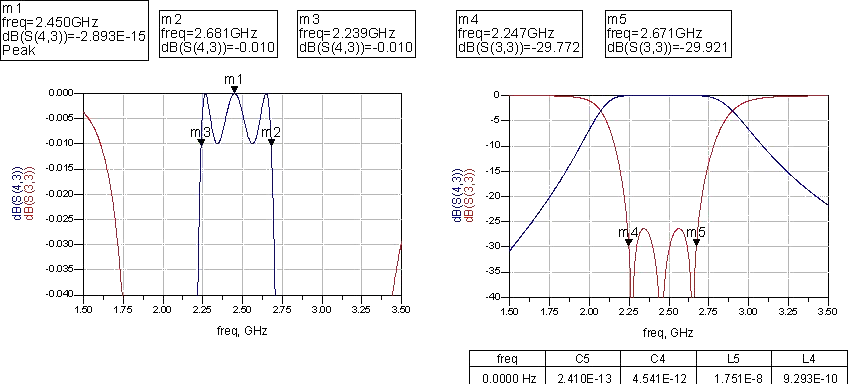
\includegraphics[width=15cm]{P17_simu_BP}
    \end{center}
    \caption{Réponse du filtre passe-bande}
\end{figure}

On remarque que le paramètre de réflexion a une forme opposée à celle du paramètre de transmission.

Le gabarit est bien respecté l’ondulation est bien de 0.01dB, la fréquence centrale est de 2.45GHZ,
et les fréquences de coupure de $f\pm f\times 0.09= 2.23 \& 2.67$GHz

\subsection{Résonateurs en lignes de transmission (éléments distribués)}

\begin{figure}
    \begin{center}
        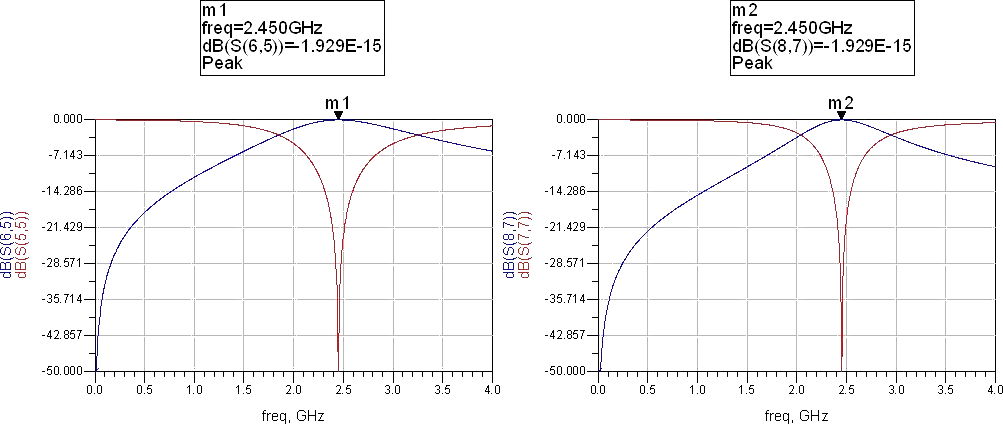
\includegraphics[width=15cm]{p17_simu_resonateur}
    \end{center}
    \caption{Simulation séparée des résonateurs}
\end{figure}

Les fréquences de résonnance des trois résonnateurs qui composent notre filtre sont \textbf{toutes} de 2.45GHz.

\begin{figure}
    \begin{center}
        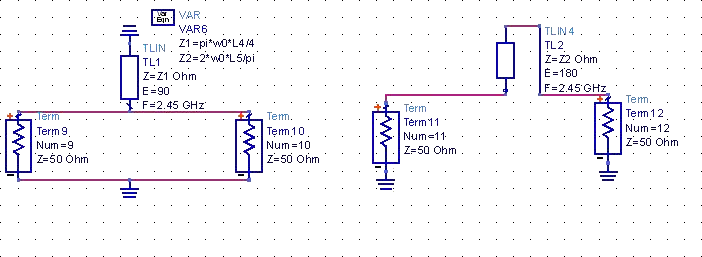
\includegraphics{p18_circuit}
    \end{center}
    \caption{Circuits et calculs des impédances de ligne}
\end{figure}

\begin{figure}
    \begin{center}
        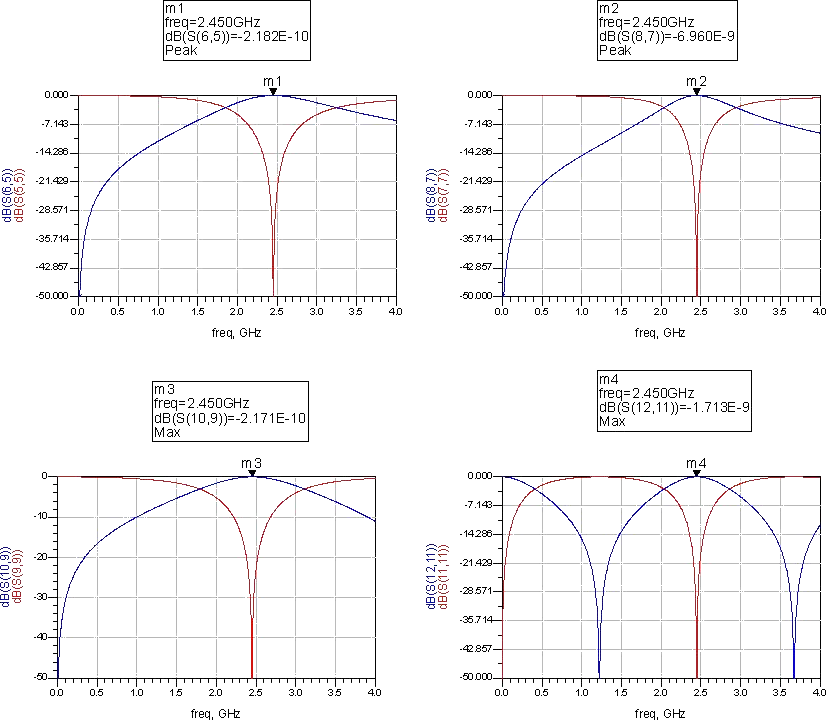
\includegraphics[width=15cm]{p18_Simu}
    \end{center}
    \caption{Simulation séparée des résonateurs des modèles localisés et de leurs équivalents en lignes de transmission}
\end{figure}

On remarque que les modèles en lignes de transmission sont identiques aux modèles localisés, si ce n’est
qu’ils périodisent le spectre.

$Z=Z_0\cfrac{Z_C+jZ_0\tan{E}}{Z_0+jZ_C\tan{E}}$, donc pour E=90°,
$Z=Z_0\cfrac{\cfrac{Z_C}{\tan{E}}+jZ_0}{\cfrac{Z_0}{\tan{E}}+jZ_C} = \cfrac{Z_0^2}{Z_C}$ ; et pour E=180°,
$Z=Z_0\cfrac{Z_C}{Z_0} = Z_C$.

\begin{figure}
    \begin{center}
        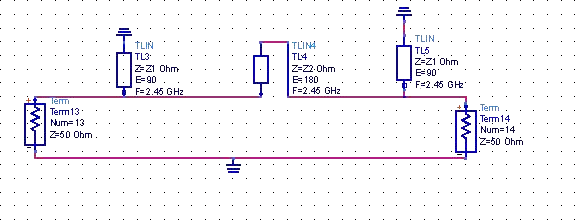
\includegraphics{p19_circuit}
    \end{center}
    \caption{Filtre en éléments distribués idéaux}
\end{figure}

\begin{figure}
    \begin{center}
        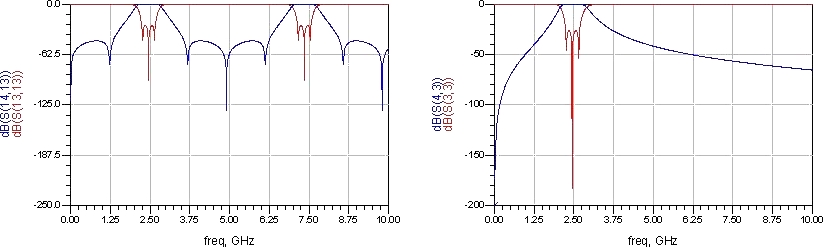
\includegraphics[width=15cm]{p19_Simu}
    \end{center}
    \caption{Comparation des réponses des filtres en éléménts distribués idéaux et en éléments localisés}
\end{figure}

On remarque une fois de plus une périodisation du spectre induite par les éléments distribués idéaux.

\begin{figure}
    \begin{center}
        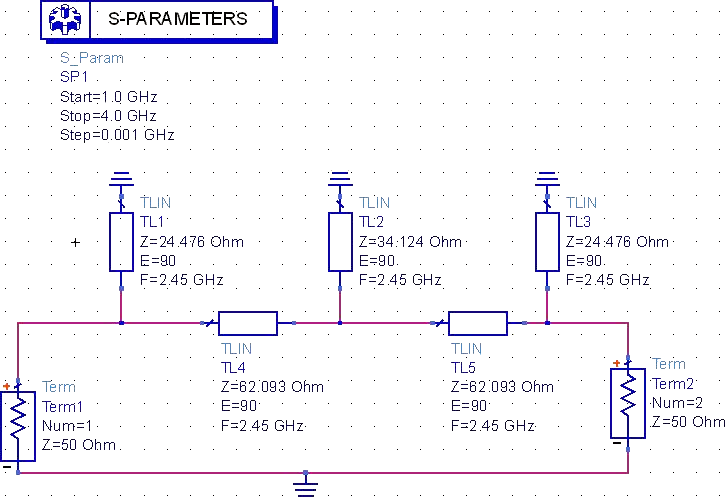
\includegraphics[width=15cm]{p19_circuit2}
    \end{center}
    \caption{Filtre passe-bande à stubs CC}
\end{figure}

\begin{figure}
    \begin{center}
        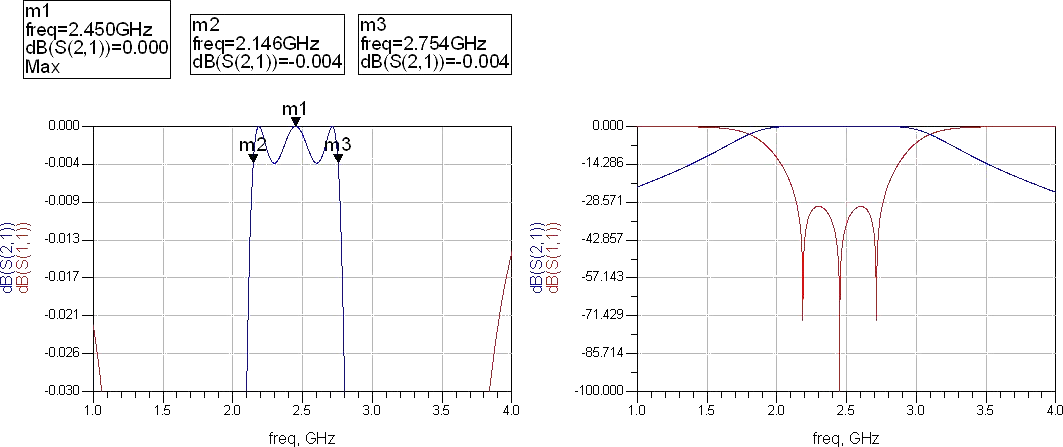
\includegraphics[width=15cm]{p19_Simu2}
    \end{center}
    \caption{Réponse du filtre passe-bande à stubs CC}
\end{figure}

Comme l’indiquent les curseurs, la bande passante du filtre est de $2754-2145=608$MHz, le Ripple est de 0.004dB et la fréquence centrale de 2.45GHz

\subsection{Passage en technologie}

Pour connaitre la gamme d’impédances réalisables dans cette technologie, on utilise l’outil \verb|LineCalc| :

\begin{figure}
    \begin{center}
        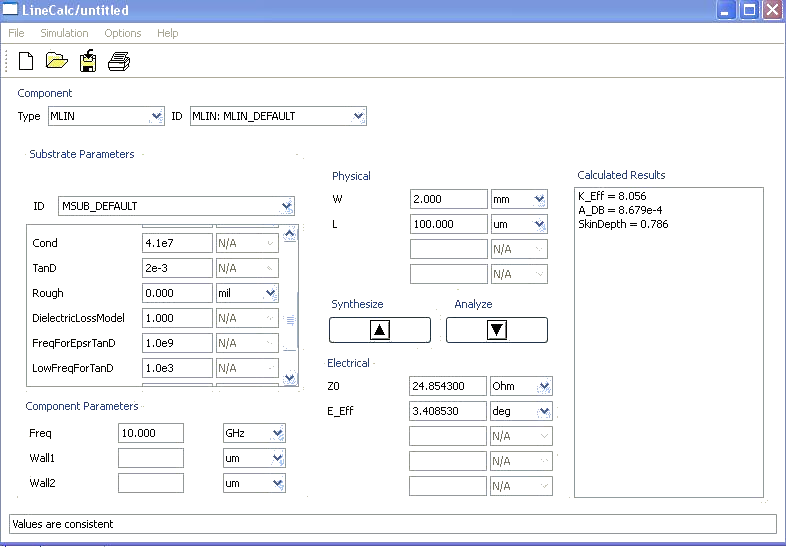
\includegraphics[width=15cm]{p20_2}
    \end{center}
    \caption{Calcul de l’impédance à 2mm}
\end{figure}
\begin{figure}
    \begin{center}
        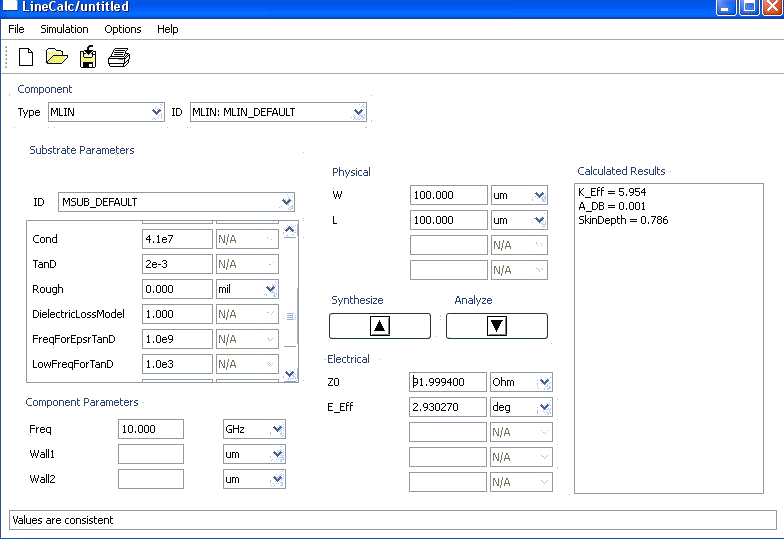
\includegraphics[width=15cm]{p20_100}
    \end{center}
    \caption{Calcul de l’impédance à 100 µm}
\end{figure}

Cette gamme d’impédance va donc de 25 à 90 $\Omega$.

Compte tenu des impédances du filtre (24, 34 et 62 $\Omega$), il est possible de le réaliser (de justesse…).

On calcule donc les longueurs et largeurs des lignes:

\begin{figure}
    \begin{center}
        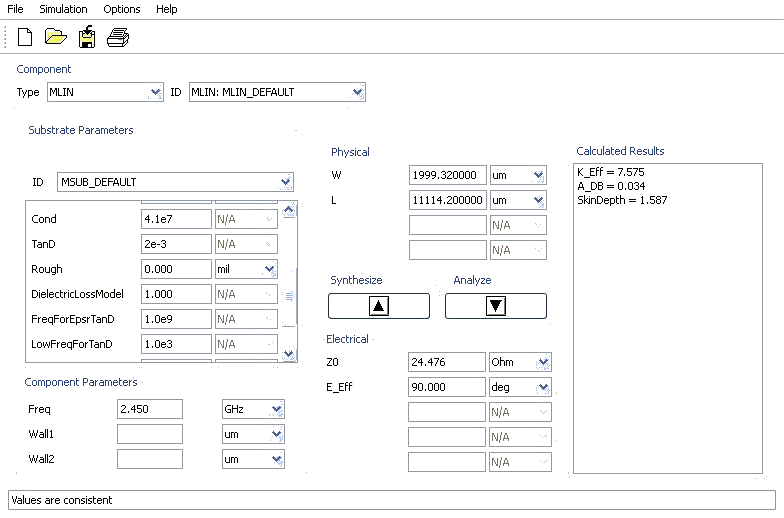
\includegraphics[width=15cm]{p21_W1_L1}
    \end{center}
    \caption{Calcul de W1 \& L1}
\end{figure}

\begin{figure}
    \begin{center}
        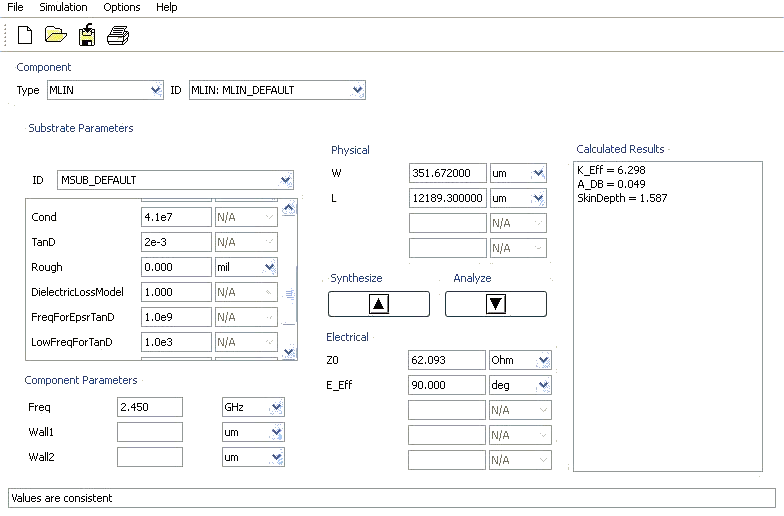
\includegraphics[width=15cm]{p21_W2_L2}
    \end{center}
    \caption{Calcul de W2 \& L2}
\end{figure}

\begin{figure}
    \begin{center}
        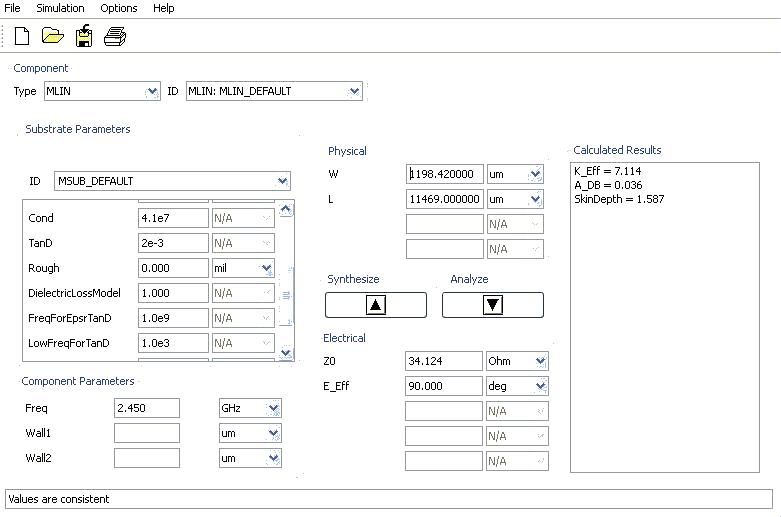
\includegraphics[width=15cm]{p21_W3_L3}
    \end{center}
    \caption{Calcul de W3 \& L3}
\end{figure}

\begin{figure}
    \begin{center}
        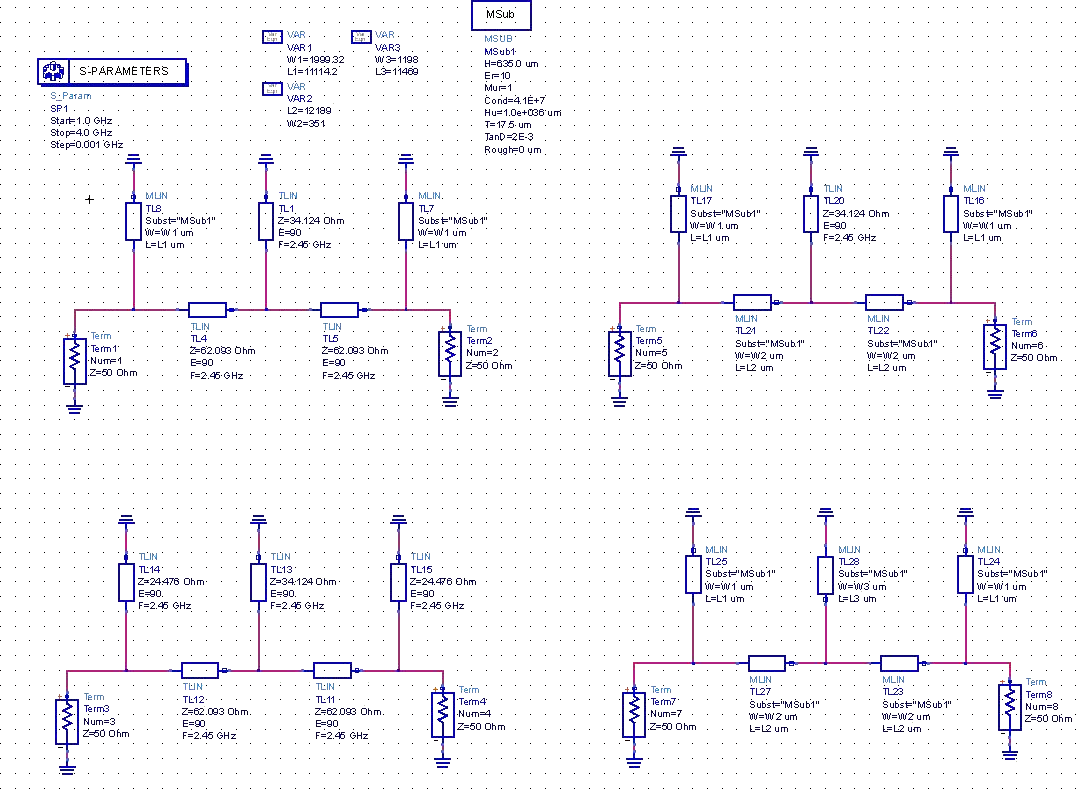
\includegraphics[width=15cm]{p21_Circuit}
    \end{center}
    \caption{Passage en technologie: Circuits des différentes étapes après «Tunage»}
\end{figure}

\begin{figure}
    \begin{center}
        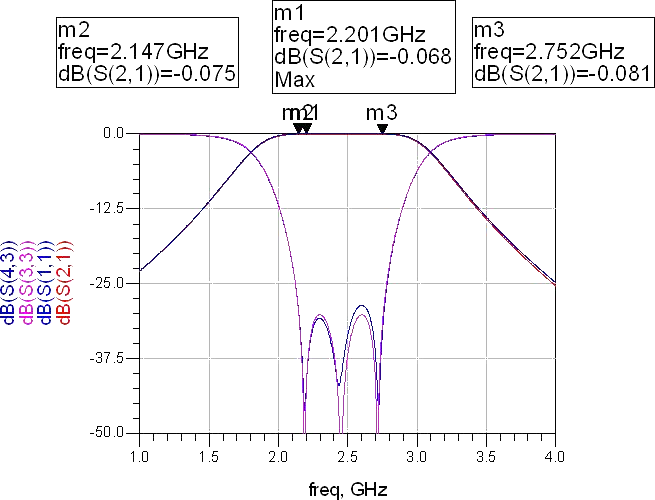
\includegraphics[width=14cm]{p21_Simu}
    \end{center}
    \caption{Passage en technologie: Réponse après la première étape}
\end{figure}
\begin{figure}
    \begin{center}
        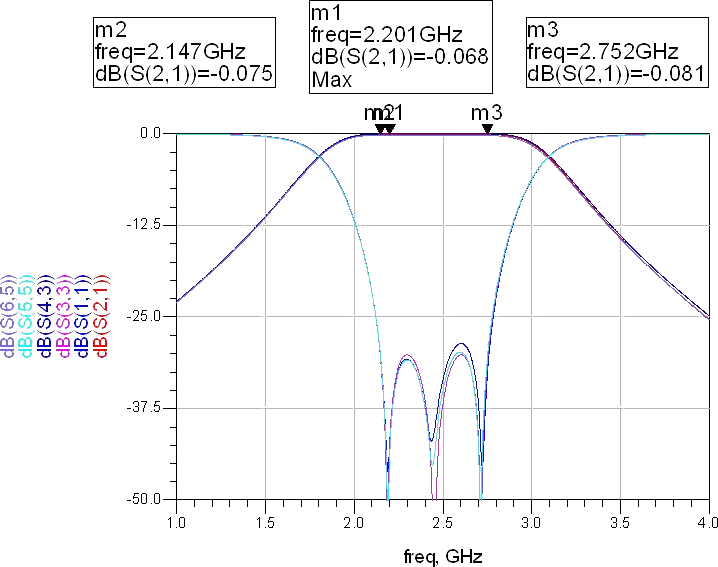
\includegraphics[width=14cm]{p21_Simu2}
    \end{center}
    \caption{Passage en technologie: Réponse après la deuxième étape}
\end{figure}
\begin{figure}
    \begin{center}
        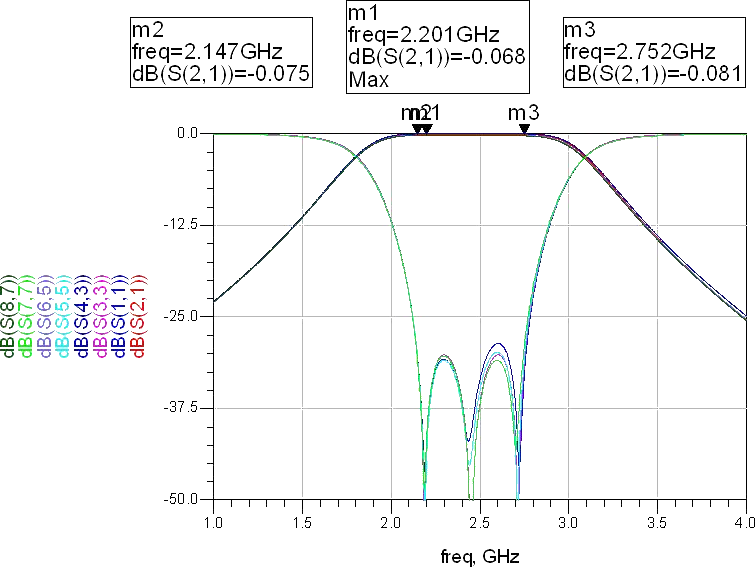
\includegraphics[width=14cm]{p21_Simu3}
    \end{center}
    \caption{Passage en technologie: Réponse après la troisième étape}
\end{figure}


Une fois le filtre réglé, nous ajoutons (petit à petit) les discontinuités en T:

\begin{figure}
    \begin{center}
        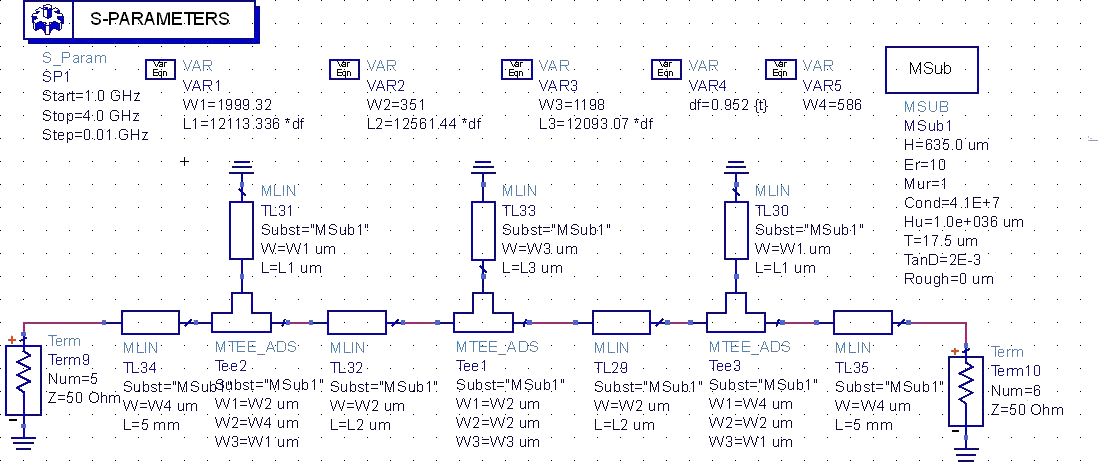
\includegraphics[width=15cm]{last_circuit}
    \end{center}
    \caption{Ajout des discontinuités en T sur le circuit}
\end{figure}

Bien sûr, ceci casse tout et il faut reprendre les réglages. La preuve:

\begin{figure}
    \begin{center}
        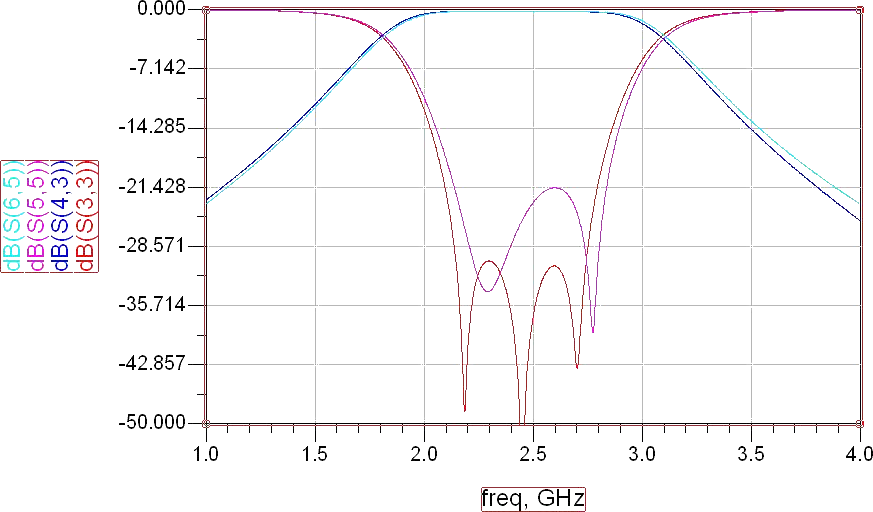
\includegraphics[width=15cm]{p22_Simu_sans_tune}
    \end{center}
    \caption{Impact de l’ajout des discontinuités en T}
\end{figure}

Mais après un nouveau réglage, on obtient à nouveau un filtre satisfaisant:

\begin{figure}
    \begin{center}
        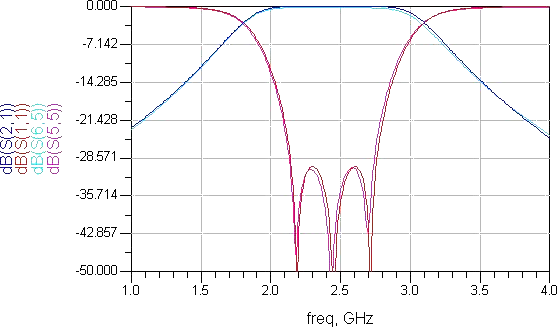
\includegraphics[width=15cm]{p22_Simu_avec_tune}
    \end{center}
    \caption{Réponse du filtre prenant correctement en compte les discontinuités}
\end{figure}

\subsection{génération de masque et Simulation électromagnétique MOMENTUM}

\begin{figure}
    \begin{center}
        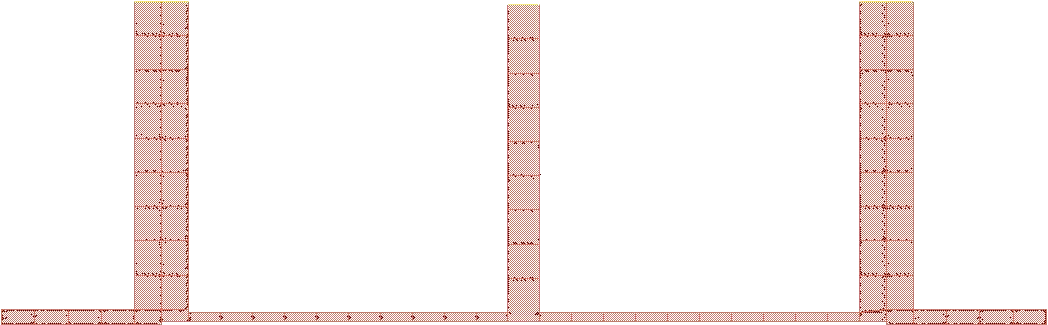
\includegraphics[width=15cm]{typon-white}
    \end{center}
    \caption{Typon}
\end{figure}

\begin{figure}
    \begin{center}
        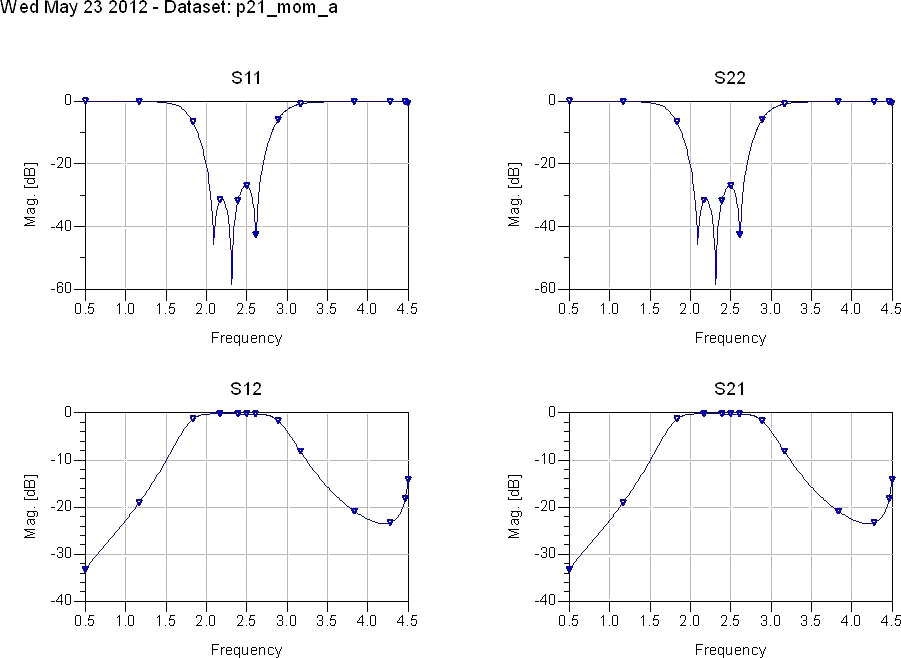
\includegraphics[width=14cm]{last_simu}
        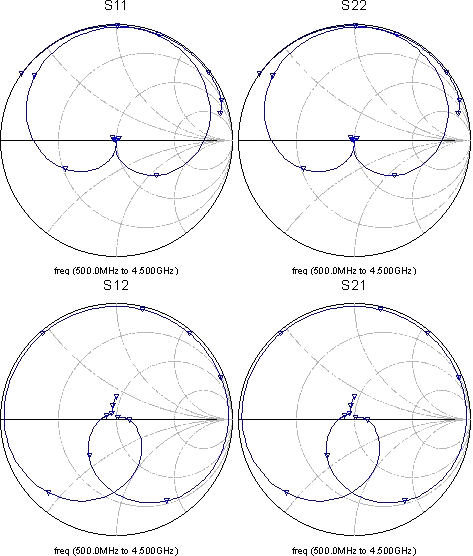
\includegraphics{last_simu2}
    \end{center}
    \caption{Réponse du Typon}
\end{figure}

\end{document}
